\section{Plumbing}\label{sec:plumbing}

In the previous section, we constructed homotopy spheres as boundaries of total spaces of disk bundles. This is a beautiful, geometric construction of exotic spheres, relying on some exceptional isomorphisms of low-dimensional Lie groups and the topology of the Hopf bundles.
However, this construction has several disadvantages.
The biggest disadvantage is the homotopy theoretic obstructions to extending the construction outside of the dimensions $1,3,7,$ and $15$. Unless we were extremely lucky and these and dimensions were the only ones containing exotic spheres, we are in need of a more flexible construction.

In this section we introduce the plumbing construction, which allows for the construction of a highly-connected manifold with a given even $(-1)^m$-symmetric unimodular intersection form with boundary a homotopy sphere. All such homotopy spheres are shown to be in $\bP^{2m}$. In fact, it turns out that all homotopy spheres in $\bP^{2m}$ can be constructed with the plumbing construction.
There are a few good sources on plumbing, ranging in abstraction and generality. A very thorough treatise is Chapter~V of \cite{browder1972surgery}, a book on the general surgery theory of simply-connected manifolds with framings. The original description of the construction can be found in Milnor's 1958 notes \cite{milnor1958manifolds}, and a more algebraic exposition is found in Hirzebruch's notes \cite{hirzebruch1971quadratic}.

We begin by noting that to get manifolds in $\bP^{2m}$ of a given intersection form, the form must be even. This restricts our construction efforts somewhat.

\begin{proposition}\label{prop:intersection-form-even}
	The intersection form of a highly-connected framed $2m$-manifold is even.
\end{proposition}
\begin{proof}
	This either follows from Wu's formula for the Stiefel-Whitney classes (see Theorem 3.3 of \cite{levine1985lectures}) or by a homotopy theoretic argument (see Lemma 7  of \cite{milnor1961procedure}).
	% Let $W$ be a framed manifold. It suffices to show that the mod $2$ intersection form $\widetilde{Q}_W$ has zeroes along the diagonal, since it is the mod 2 reduction of the intersection form. For any homology class $a\in \H_{m}(W;\Z/2)$ with Poincar\'e-Lefschetz dual $\alpha\in \H^{m}(W,\partial W;\Z/2)$, we have $\widetilde{Q}_W = \alpha\smile \alpha = \Sq^m(\alpha)$, where $\Sq$ are the Steenrod operations.
	%
	% But since $W$ is highly-connected, the $m$-th Steenrod operator $\Sq^m(\alpha)=\Sq(\alpha)$ is equal to the total Steenrod operator since the other ones vanish. By \cref{sec:wu-classes}, we have $\Sq(\alpha)=v\smile \alpha$ where $v$ is the total Wu class. Since $W$ is stably parallelizable, the Wu classes are trivial and so $\widetilde{Q}^W(\alpha,\alpha)=\widetilde{Q}_W(a,a)=0$.
\end{proof}

In particular, it is important to note that the disk bundles of the previous section are not framed, since the intersection forms are $(\pm 1)$. Ultimately it turns out that the Milnor spheres do have a framed coboundary but this is not obvious from the construction.

We should also note that vector bundles over spheres behave differently outside of the dimensions in which we have a Hopf fibration. Recall that by \cref{lemma:euler-number-clutching-construction}, for rank $m$ bundles over $S^m$ the Euler number is the homomorphism
\[
	e : \pi_{m-1}(\SO_m) \lkxto \pi_{m-1}(S^{m-1}).
\]
When $m$ is odd, this map is always zero. When $m$ is even, this map has image at least $2\Z\subset \pi_{m-1}(S^{m-1})$ since the tangent bundle $\TT S^{2m}$ has Euler number $2$. However, over the spheres $S^2$, $S^4$, and $S^8$ we have the Hopf bundles of Euler number $\pm 1$, so in these cases, the image must be $\Z$. This is enough for a full description of the image of $e$.

\begin{proposition}\label{thm:possible-euler-numbers-over-spheres}
	The Euler number map $e : \pi_{m-1}(\SO_m) \to \pi_{m-1}(S^{m-1})$ has image
	\[
		e : \pi_{m-1}(\SO_m) \lkxto
		\begin{cases}
			\Z  & (m-1)\in\{1,3,7\},  \\
			2\Z & m\textrm{ is even}, \\
			0   & \textrm{otherwise}\end{cases}
	\]
\end{proposition}
\begin{proof}
	See Section 1 of \cite{levine1985lectures}.
\end{proof}

\subsection{Crafting an Intersection Form}

We now begin our construction.
Suppose we wish to construct a framed $2m$-dimensional manifold with a given intersection form, specified by a bilinear form $Q$ on the unit lattice $\Z^\ell$ with basis vectors $e_1,\ldots, e_\ell$. Denote this hypothetical construction by $W^{2m}$. Our construction here will allow $W$ to have a boundary, since constructing closed manifolds with a given intersection form is generally harder.

The simplest possible case is when the lattice is $1$-dimensional, with intersection form
\[
	Q =  (Q_{11})
\]
determined by the single integer $Q_{11}=Q(e_1,e_1)\in \Z$.
For the resulting manifold to have a hope of being frameable, we should require $Q_{11}$ to be even by \cref{prop:intersection-form-even}. We should also note that only the trivial bundle works in the case that $m$ is odd, since $Q$ is skew-symmetric in this case and so diagonal entries must be zero.

The resulting $2m$-manifold $W$ should have middle dimensional homology $\H_m(W)$ free of rank $1$, generated by a cycle $a$ which has self-intersection number $a \tnsv a= Q_{11}$. To construct such a manifold, we start with a $m$-dimensional sphere $S^m$. This submanifold represents the generating cycle $a\in \H_m(W)$.
To get a $2m$-dimensional manifold, we ``thicken'' the sphere by choosing a rank $m$ disk bundle $\mathcal{E} : E \to S^m$ with Euler number $Q_{11}$. Given the requirement that $Q_{11}$ is even when $m$ is even and zero when $m$ is odd, such a bundle always exists by \cref{thm:possible-euler-numbers-over-spheres}.
\begin{remark*}
	To have a consistent choice of bundle of a given even Euler number $2k$ when $m$ is even, let $\mathcal{E}$ be the bundle $k\cdot \TT S^m$, where multiplication is done in $\pi_{m-1}(\SO_m)$.
\end{remark*}
Since disks are contractible, there is a deformation retraction $E\simeq S^m$, and this implies that the middle dimensional homology $\H_m(E)$ is generated by $a$.
Then, the self intersection number of $a$ is exactly the Euler number $e(\mathcal{E})$.
We can then define $W$ as the total space $E$ of the disk bundle. This will be the base case for plumbing constructions.
\begin{figure}[ht]
	\centering
	\import{diagrams}{thickening-sphere.pdf_tex}
	\caption{Two different ``thickenings'' of $S^1$ by $D^1$ bundles.}\label{fig:thickening-sphere}
\end{figure}
\begin{remark*}
	Although plumbing non-orientable bundles is certainly possible and interesting in its own right, to keep the resulting manifolds orientable we'll require orientable bundles $\mathcal{E}$ (this rules out the M\"obius bundle thickening in \cref{fig:thickening-sphere}). With this requirement, $W$ gets a manifold orientation from the orientation of the bundle.
\end{remark*}

\begin{remark*}
	Note that this base case is defined similarly to the Milnor manifolds, namely as the boundary of a disk bundle over a sphere. However, the requirement that the Euler number is even means that the plumbed manifold associated to a 1-dimensional intersection form can never be a homotopy sphere by \cref{prop:homotopy-type-spherical-bundle}. In some sense, Milnor manifolds fill in the low dimensional cracks left by the much more general plumbing construction.
\end{remark*}
\subsection{Plumbing Multiple Bundles}

Let us now consider the case of a $2$-dimensional lattice, and try to construct a manifold with intersection form $Q$ given by the $2\times 2$ integer matrix:
\[
	Q = \begin{pmatrix} Q_{11} & Q_{12} \\ Q_{21} & Q_{22}\end{pmatrix}.
\]
This matrix should be even and $(-1)^m$-symmetric. To begin constructing a manifold, we want $\H_m(W)$ to be free of rank $2$, generated by cycles $a$ and $b$ with intersection numbers specified by the matrix $Q$.
The simplest case is when $|Q_{12}|=|Q_{21}|=0$, i.e. the intersection forms is represented by a diagonal matrix and splits as a direct sum $Q=Q_1\oplus Q_2$. In this case by \cref{prop:connected-sum-intersection-form}, we can define
\[
	P(Q_1\oplus Q_2) = P(Q_1)\+ P(Q_2).
\]
In fact, this construction lets us realize any diagonal matrix as the intersection form of a manifold, assuming all entries along the diagonal are even.

The next simplest case is when $|Q_{12}|=|Q_{21}|=1$. We want the cycles $a$ and $b$ to intersect exactly once. We start with a wedge of two spheres $S^m_1\vee S^m_2$ representing $a$ and $b$ respectively. Next we thicken this space into a $2m$-dimensional space by choosing rank $m$ bundles $\mathcal{E}_i : E_i \to S^m_i$ with Euler numbers $Q_{i,i}$. To get rid of the singularity at the attachment point, we perform some identifications in a ``criss-cross'' manner.

\begin{figure}[ht]
	\centering
	\import{diagrams}{plumbing-two-circles-smoothed.pdf_tex}
	\caption{A plumbing of two trivial bundles.}\label{fig:plumbing-two-circles}
\end{figure}

If $S^m_1$ and $S^m_2$ are wedged together at points $x_1$ and $x_2$,
the bundles $D(\mathcal{E}_i)$ admit local trivializations on a tubular neighborhood $D^m \subset S^m_i$ of the point $x_i$, i.e. a disk.
Since the fibers are also $D^m$, we get smooth embeddings of pairs $(D^m\times D^m, \partial D^m\times D^m)\subset (D(E_i),\partial D(E_i))$.
Now we can identify the first disk factor of the first bundle with the second disk factor of the second bundle, and the second disk factor of the first bundle with the first disk factor of the second bundle (see \cref{fig:plumbing-two-circles} for an example). After smoothing out the corners, as described in \cref{rmk:smoothing-corners}, we get a smooth manifold in which $S_1^m$ and $S_2^m$ intersect transversally exactly once at $x_1=x_2$. More generally:

\begin{definition}\label{def:plumbing}
	Let $W_1$ and $W_2$ be manifolds with orientation preserving embeddings\,\footnote{Note that these are not neat embeddings, as is assumed for submanifolds throughout this thesis.}
	\[\iota_i : (D^m\times D^m, \partial D^m\times D^m)\lkxto (W_i, \partial W_i).\]
	The \defn{plumbing} of $W_1$ and $W_2$, denoted by $W_1\plumb W_2$, is the quotient space
	\[
		W_1\plumb W_2 = \frac{W_1\sqcup W_2}{\iota_1(x,y)\sim \iota_2(y,x).}
	\]
\end{definition}

\begin{remark*}\label{rmk:smoothing-corners}
	The plumbing has an a priori smooth structure everywhere except at the corners which arise from the boundaries $\partial D^m\times \partial D^m$ in $W_1\plumb W_2$. The usual approach of smoothing corners applies here, see \cref{sec:smoothing-corners} for a brief discussion.
\end{remark*}

\begin{remark*}
	Since $D^m\times D^m$ is a tubular neighborhood of both $\{0\}\times D^m$ and $D^m\times\{0\}$, the plumbing of two disk bundles can be thought of as a join along an embedded fiber $D^m$ of $E_1$ and an chart $D^m\subset S^m\subset E_2$. Of course, the latter of these is not a (neat) submanifold because the boundary of $D^m$ maps to the interior of $E_2$. Consequently, there needs to be an additional step to smooth out the corners.
\end{remark*}

Now we study the intersection theory of the plumbed manifold. It is clear that the submanifolds $S_1^m$ and $S_2^m$ intersect transversally at a single point. The sign is determined by the orientation of horizontal and vertical disks in the embedding $\iota_i$. In particular, if we precompose $\iota_2$ by the product $D^m\times D^m\to D^m\times D^m$ of two orientation-reversing maps, the orientation of the plumbing reverses. For disk bundles $D(E_1)$ and $D(E_2)$, let us normalize the plumbing so that the intersection number $a\cdot b$ is $+1$ when we write $D(E_1)\plumb D(E_2)$, and $a\cdot b$ is $-1$ when we write $D(E_1)\plumb^{-1} D(E_2)$.

Next, we investigate how plumbing affects a framing.
Suppose $S_1^m$ and $S_2^m$ are spheres, with bundles $\mathcal{E}_1 = k_1\cdot \TT S^m$ and $\mathcal{E}_2=k_2\cdot \TT S^m$. Let $P=D(E_1)\plumb D(E_2)$ be the resulting plumbing. We have a decomposition
	\begin{equation}\label{eq:plumbing-tangent-decomposition}
		\TT P|_{D(E_i)} = \TT S^m_i\oplus k\cdot \TT S^m
	\end{equation}
	Since any sphere $S^m$ has a framing given by the unit normal field in $\R^{m+1}$, the bundle $\TT S^m\oplus\underline{\R}^1$ is trivial.
	It follows from \cref{eq:plumbing-tangent-decomposition} that $\TT P\oplus \underline{\R}^1|_{D(E_i)}$ is trivial, and so $\TT P|_{S_i^m}$ is trivial. Since we constructed the manifold to be orientable, these trivializations are compatible and so it follows that $\TT P|_{S_1^m\vee S_2^m}$ is trivial. Since there is a homotopy equivalence $P\simeq S_1^m\vee S_2^m$, it follows that $\TT P$ is trivial as well. Consequently, $P$ admits a framing. 
	% see \cref{fig:framing-of-plumbed-manifold} for a visual example.
	% \begin{figure}[ht]
	% 	\centering
	% 	\import{diagrams}{framing-on-plumbing.pdf_tex}
	% 	\caption{Framing on a plumbing}\label{fig:framing-of-plumbed-manifold}
	% \end{figure}

Note that plumbing is an entirely local operation, so by choosing distinct embeddings we can plumb together multiple disk bundles, or plumb together two bundles at multiple points. Furthermore, each plumbing point introduces a single transverse intersection, affecting the global intersection number of a generating sphere by $\pm 1$.
\begin{figure}[ht]
	\centering
	\import{diagrams}{plumbing-multiple-points.pdf_tex}
	\caption{Plumbing two bundles at multiple points.}\label{fig:plumbing-at-multiple-points}
\end{figure}
We can therefore plumb together two bundles at multiple points with local intersection numbers either $+1$ or $-1$ to get an any integer global intersection number. See \cref{fig:plumbing-at-multiple-points} for an example. However, we must be careful to either plumb all points with positive orientation or all points with negative orientation. This ensures the manifold remains orientable and that the framing extends over the new plumbed region.

\begin{proposition}\label{thm:plumbing-existence-theorem}
	For $m>1$ and $Q$ any even, $(-1)^m$-symmetric, and indecomposable\,\footnote{This assumption removes a slight ambiguity from the statement of this theorem. Whenever there is a decomposition $Q=A\oplus B$, we can either take the connected sum $P^{2m}(A)\+P^{2m}(B)$ or boundary connected sum to get $(P^{2m}(A),\partial P^{2m}(A))\+ (P^{2m}(B),\partial P^{2m}(B))$ depending on our goals.} form, there is a highly-connected framed $2m$-manifold $P^{2m}(Q)$ with intersection form $Q$.
\end{proposition}

\begin{proof}
Let $\Lambda$ be the lattice on which $Q$ is defined, and assume we have a basis $\{e_1,\ldots, e_\ell\}$. To construct $P^{2m}(Q)$, start with spheres $S_1^m=S^m,\ldots, S_\ell^m=S^m$, and take the bundles $\mathcal{E}_1=(Q_{11}/2)\cdot \TT S^m_1,\ldots, \mathcal{E}_\ell=(Q_{\ell\ell}/2)\cdot \TT S^m_1$. Then for every $i<j$, we plumb together $D(E_i)$ with $D(E_j)$ with multiplicity $Q_{i,j}$, resulting in $P^{2m}(Q)$. When off-diagonal entries $Q_{i,j}$ are not $0$ or $\pm 1$, the constructed manifold is no longer simply-connected, and surgery is required to keep the manifold highly-connected. 

We defer these technicalities to Section V.2 of \cite{browder1972surgery}.
\end{proof}

For our purposes, we will only need to construct manifolds whose intersection forms have diagonal entries $\pm 2$ and off-diagonal entries $\{0,\pm 1\}$, and we only include the more general results for completeness. We could therefore assume that all bundles are $\pm \TT S^m$ and that two bundles are plumbed together at at most $1$ point.
%
% 	Under a contraction of fibers, it is clear $P^{2m}(Q)$ deformation retracts onto a disjoint union of the spheres $S^m_i$ which are pairwise wedged together at $|Q_{ij}|$ points. We would like to simplify this homotopy type. First, we note that:
% 	\begin{lemma}
% 		For each integer $q\geq 1$, there is a homotopy equivalence
% 		\[
% 			S^m\vee^q S^m \simeq S^m\vee S^m \vee \bigvee_{q-1} S^1,
% 		\]
% 		where $S^m\vee^q S^m$ denotes the wedge sum of two $m$-spheres at $q$ points.
% 	\end{lemma}
%
% 	In particular, this means that $P^{2m}(Q)$ admits a deformation retract onto the space
% 	\[
% 		\underbrace{S^m\vee\cdots S^m}_{\ell}\vee \bigvee_N S^1.
% 	\]
% 	for some large enough $N$. It follows that $\H^m(P^{2m}(Q))$ is free abelian of rank $\ell$ (here the assumption that $m>1$ is useful) and that the intersection form of $P^{2m}(Q)$ is exactly $Q$. Furthermore, we get a framing on $P^{2m}(Q)$ by \cref{rmk:plumbing-framing}.
The remaining work involves understanding the homotopy type of the boundary. 

\begin{proposition}\label{prop:fundamental-group-plumbing}
	There is a surjective map
	\[\pi_1(\partial P^{2m}(Q))\lkxsurj \pi_1(P^{2m}(Q))\]
	with the latter group free. For $m>2$, the map is an isomorphism.
\end{proposition}
\begin{proof}
	See Lemma V.2.4 of \cite{browder1972surgery}.
\end{proof}

\begin{theorem}
	If $Q$ is unimodular, then $\partial P^{4m}(Q)$ is a homotopy sphere in $\bP^{4m}$.
\end{theorem}
\begin{proof}
	See Theorem V.2.1 of \cite{browder1972surgery}.
\end{proof}

At this point, we can recall the $\E_8$ form defined in \cref{sec:intersection-form-invariants}. Since this is an even unimodular form, plumbing along this matrix gives:
\begin{theorem}\label{thm:plumbing-theorem}
	There is a group homomorphism
	\[
		\lkxfunc{}{\Z}{\bP^{4k}}{n}{\partial P^{4k}(E_8)\+\cdots\+\partial P^{4k}(E_8),}
	\]
	where the boundary of each sphere is a highly-connected manifold of signature $8n$.
\end{theorem}

This is a weaker form of the plumbing theorem (Theorem V.2.9 of \cite{browder1972surgery}), which also constructs a framed homotopy equivalence $(P^{4k}(\E_8), \partial P^{4k}(\E_8)) \to (D^{4k}, S^{4k-1})$.

\begin{remark*}
	When $k=1$, the $E_8$ plumbing $\partial P^{4}(E_8)$ does not give a homotopy $3$-sphere, but rather a homology $3$-sphere $\mathscr{D}$ known as the \defn{Poincar\'e homology sphere} or dodecahedral space. This space has fundamental group $\pi_1(\mathscr{D})$ of order 120, a preimage of $A_5$ under the double cover $\SU_2 \to \SO_3$. 
	This group is perfect, meaning it has trivial abelianization and so $\H^1(\mathscr{D})\cong \pi_1(\mathscr{D})/[\pi_1(\mathscr{D}), \pi_1(\mathscr{D})]\cong 0$ by the Hurewicz isomorphism.
		

\begin{figure}[ht]
	\centering
	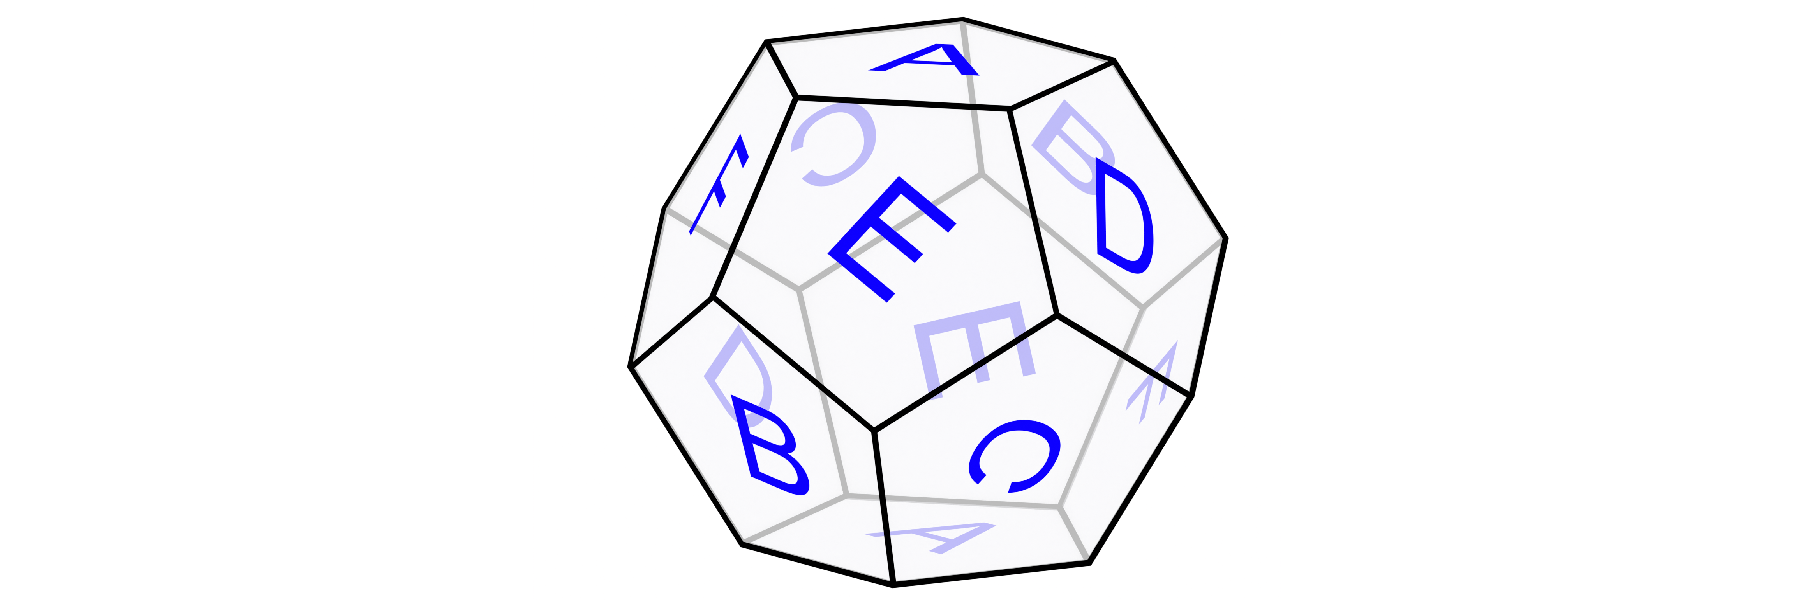
\includegraphics[height=1.5in]{diagrams/dodecahedral-space-geometric-construction.png}
	\caption{Construction of Dodecahedral Space}\label{fig:dodecahedral_space_construction}
\end{figure}

	The classic construction of dodecahedral space $\mathscr{D}$ is due to Poincar\'e. Note that the solid dodecahedron has 6 pairs of opposite pentagonal faces. Picking a clockwise spherical orientation on $\mathscr{D}$, we can glue together opposing faces with a minimal clockwise twist to line them up (see \cref{fig:dodecahedral_space_construction}). The resulting quotient space is the closed $3$-manifold $\mathscr{D}$.

	Since $\mathscr{D}$ violates Poincar\'e's original (incorrect) hypothesis that every homology $3$-sphere is homeomorphic to the $S^3$, the Poincar\'e dodecahedral space might be referred to as a ``proto'' exotic sphere. For some equivalent perspectives on dodecahedral space, including proofs of equivalences with the $\E_8$ plumbing, see \cite{kirby1979eight}.
\end{remark*}

\subsection{Graphs and Integral Bilinear Forms}
We close our discussion of the plumbing construction with a convenient bit of notation which simplifies the often large matrices which arise when plumbing manifolds. Particularly, matrices such as the $E_8$ matrix can be viewed as a matrix associated to a weighted graph.
This connection between plumbing matrices and graphs was noticed by Hirzebruch.

\begin{definition}
	A \defn{graph} $G$ is a finite connected $1$-dimensional simplicial complex.
	A \defn{weighted graph}[graph (weighted)] is a pair $(G,w)$ consisting of a graph $G$ and a map $w : \Vert(G) \to \Z$ assigning a \defn{weight} $w(v)\in \Z$ to each vertex $v$ of the graph.
\end{definition}

Given a graph $G$ with vertices $\{e_1,\ldots, e_\ell\}$ and integral weights $w$, the matrix associated to $G$ is the $(-1)^m$-symmetric matrix given by
\[
	Q_{ij} = \begin{cases}
		w(e_i)    & i=j,                       \\
		(\pm 1)^m & (i,j)\in \textrm{Edge}(T), \\
		0         & \textrm{otherwise}.
	\end{cases}
\]
In the skew-symmetric case, we adopt the convention that the upper-triangular part of the matrix is positive. Note that the matrix corresponding to a (connected) graph is indecomposable.

\begin{remark*}
If $Q$ is a matrix associated to a graph $G$, the plumbing $P(Q)$ has a $1$-skeleton which is homotopy equivalent to $G$.
\end{remark*}

\begin{remark*}
	There are various modifications of this notion in the literature. For instance, in Section~8 of \cite{hirzebruch1971quadratic}, plumbings along a graph with weights in the group $\pi_{m-1}(\SO_m)$ instead of $\Z$ are considered.
\end{remark*}


\begin{definition}
	A \defn{tree} is a simply-connected graph, i.e. a graph with no cycles.
\end{definition}

\begin{figure}[ht]
	\centering
	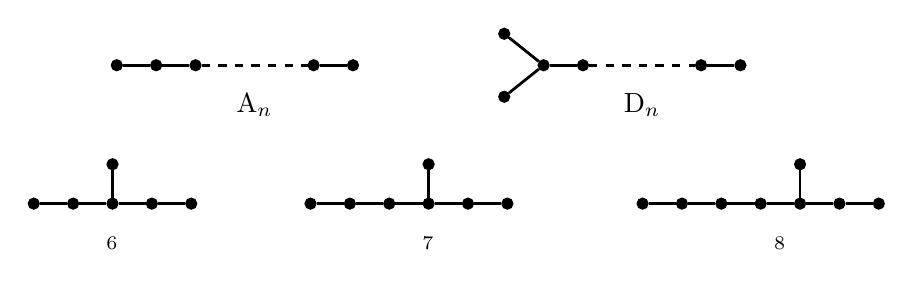
\begin{tikzpicture}
		\tikzset{dynode/.style={circle, draw, fill=black,
					minimum size=4pt, inner sep=0pt}}
		\tikzset{dyline/.style={line width=1pt}}
		\tikzset{dydash/.style={line width=1pt, dashed}}

		\begin{scope}[yshift=0, xshift=22em]
			\node[dynode] (a1) at (0,0) {};
			\node[dynode] (a2) at (0.5,0) {};
			\node[dynode] (a3) at (1,0) {};
			\node[dynode] (a4) at (1.5,0) {};
			\node[dynode] (a5) at (2,0) {};
			\node[dynode] (a6) at (2.5,0) {};
			\node[dynode] (a7) at (3,0) {};
			\node[dynode] (a8) at (2,0.5) {};

			\draw[dyline] (a1) -- (a2) -- (a3) -- (a4) -- (a5) -- (a6) -- (a7);
			\draw[dyline] (a5) -- (a8);

			\node[] (l) at (1.75,-0.5) {$\E_8$};
		\end{scope}

		\begin{scope}[yshift=0, xshift=10em]
			\node[dynode] (a1) at (0,0) {};
			\node[dynode] (a2) at (0.5,0) {};
			\node[dynode] (a3) at (1,0) {};
			\node[dynode] (a4) at (1.5,0) {};
			\node[dynode] (a5) at (2,0) {};
			\node[dynode] (a6) at (2.5,0) {};
			\node[dynode] (a8) at (1.5,0.5) {};

			\draw[dyline] (a1) -- (a2) -- (a3) -- (a4) -- (a5) -- (a6);
			\draw[dyline] (a4) -- (a8);

			\node[] (l) at (1.5,-0.5) {$\E_7$};
		\end{scope}

		\begin{scope}[yshift=0, xshift=0]
			\node[dynode] (a1) at (0,0) {};
			\node[dynode] (a2) at (0.5,0) {};
			\node[dynode] (a3) at (1,0) {};
			\node[dynode] (a4) at (1.5,0) {};
			\node[dynode] (a5) at (2,0) {};
			\node[dynode] (a8) at (1,0.5) {};

			\draw[dyline] (a1) -- (a2) -- (a3) -- (a4) -- (a5);
			\draw[dyline] (a3) -- (a8);

			\node[] (l) at (1,-0.5) {$\E_6$};
		\end{scope}

		\begin{scope}[yshift=5em, xshift=3em]
			\node[dynode] (a1) at (0,0) {};
			\node[dynode] (a3) at (0.5,0) {};
			\node[dynode] (a4) at (1,0) {};
			\node[dynode] (a5) at (2.5,0) {};
			\node[dynode] (a6) at (3.0,0) {};

			\draw[dyline] (a1) -- (a3) -- (a4);
			\draw[dydash] (a4) -- (a5);
			\draw[dyline] (a5) -- (a6);

			\node[] (l) at (1.75,-0.5) {$\mathrm{A}_n$};
		\end{scope}

		\begin{scope}[yshift=5em, xshift=17em]
			\node[dynode] (a1) at (0,0.4) {};
			\node[dynode] (a2) at (0,-0.4) {};
			\node[dynode] (a3) at (0.5,0) {};
			\node[dynode] (a4) at (1,0) {};
			\node[dynode] (a5) at (2.5,0) {};
			\node[dynode] (a6) at (3.0,0) {};

			\draw[dyline] (a1) -- (a3);
			\draw[dyline] (a2) -- (a3);
			\draw[dyline] (a3) -- (a4);
			\draw[dydash] (a4) -- (a5);
			\draw[dyline] (a5) -- (a6);

			\node[] (l) at (1.75,-0.5) {$\mathrm{D}_n$};
		\end{scope}
	\end{tikzpicture}
	\vspace{1em}
	\caption{Dynkin diagrams associated to simple Lie groups.} \label{fig:dynkin-diagram-trees}
\end{figure}

A rich source of trees by which to construct plumbed manifolds are the Dynkin diagrams associated to root systems, see \cref{fig:dynkin-diagram-trees} for the complete set of undirected Dynkin diagrams. There is a deep connection between Dynkin diagrams and the classification of simple Lie groups -- $\mathrm{A}_n$ corresponds to $\SU_{n+1}$, $\mathrm{D}_n$ corresponds to $\SO_{2n}$, and $\E_6, \E_7, \E_8$ correspond to exceptional Lie groups of dimensions 78, 133, and 248 respectively.
A complete discussion of this beautiful topic would take us too far afield, so we refer to Chapter~21 of Fulton and Harris's book \cite{fultonharris1991representation} or to Chapter~3 of Humphrey's book \cite{humphreys1972representation}.

\begin{example}
	If we weight each vertex by $2$, the symmetric bilinear form associated to the $\E_8$ Dynkin diagram has the matrix form
	\[
		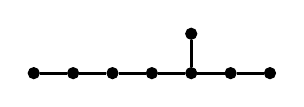
\begin{tikzpicture}
			\tikzset{dynode/.style={circle, draw, fill=black,
						minimum size=4pt, inner sep=0pt}}
			\tikzset{dyline/.style={line width=1pt}}
			\tikzset{dydash/.style={line width=1pt, dashed}}

			\begin{scope}[yshift=-10em, xshift=0]
				\node[dynode] (a1) at (0,0) {};
				\node[dynode] (a2) at (0.5,0) {};
				\node[dynode] (a3) at (1,0) {};
				\node[dynode] (a4) at (1.5,0) {};
				\node[dynode] (a5) at (2,0) {};
				\node[dynode] (a6) at (2.5,0) {};
				\node[dynode] (a7) at (3,0) {};
				\node[dynode] (a8) at (2,0.5) {};

				\draw[dyline] (a1) -- (a2) -- (a3) -- (a4) -- (a5) -- (a6) -- (a7);
				\draw[dyline] (a5) -- (a8);
			\end{scope}
		\end{tikzpicture}
		\quad\lkxto\quad
		\begin{pmatrix}
			2 & 1 &   &   &   &   &   &   \\
			1 & 2 & 1 &   &   &   &   &   \\
			  & 1 & 2 & 1 &   &   &   &   \\
			  &   & 1 & 2 & 1 &   &   &   \\
			  &   &   & 1 & 2 & 1 &  & 1 \\
			  &   &   &   & 1 & 2 & 1 &  \\
			  &   &   &   &  & 1 & 2 &  \\
			  &   &   &   & 1 &  &  & 2 \\
		\end{pmatrix}.
	\]	
\end{example}

\subsection{The Kervaire Sphere}

Thus far, the
	\[
		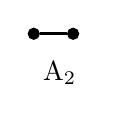
\begin{tikzpicture}
			\tikzset{dynode/.style={circle, draw, fill=black,
						minimum size=4pt, inner sep=0pt}}
			\tikzset{dyline/.style={line width=1pt}}
			\tikzset{dydash/.style={line width=1pt, dashed}}

				\node[dynode] (a1) at (0,0.5) {};
				\node[dynode] (a2) at (0.5,0.5) {};

				\draw[dyline] (a1) -- (a2);
				\node[] (l) at (0.33,0) {$\mathrm{A}_2$};
		\end{tikzpicture}
		\quad\lkxto\quad
		\begin{pmatrix}
			0 & 1\\
			-1 & 0
		\end{pmatrix}.
	\]	

